\documentclass{article}
\usepackage{graphicx} % Required for inserting images
\usepackage{amsmath}
\usepackage{fancyhdr}
\usepackage{xcolor}
\usepackage{amsfonts} 
\usepackage{subcaption}
\usepackage{graphicx} 
\usepackage{epstopdf}
\usepackage{subcaption}
\usepackage{amssymb}
\usepackage{float}
\usepackage{textgreek}
\usepackage{fancyhdr}
\usepackage{hyperref}
\usepackage{gensymb}
\usepackage{bbm}
\usepackage[scr]{rsfso}

\newcommand{\Laplace}{\mathscr{L}}

\pagestyle{fancy}

\lhead{Pinkas Matěj}
\chead{ARI-HW\_00}
\rhead{28. February  2024}


\title{ARI-HW\_00 - Opakování SSI}
\author{Matěj Pinkas}
\date{28. February 2024}

\newcommand\mat[1]{\begin{bmatrix}#1\end{bmatrix}}
\newcommand\pmat[1]{\begin{pmatrix}#1\end{pmatrix}}
\newcommand\vmat[1]{\begin{vmatrix}#1\end{vmatrix}}
\newcommand\hw[1]{\stepcounter{section}\section*{Úkol \thesection\quad #1}}


\begin{document}

\maketitle
%----------------------------------------------------------------------------------------------------
%1
\hw{}
\begin{enumerate}
    \item Systém je stabilní když všechny jeho póly leží v záporné polorovině, tedy reálné části pólů jsou záporné.\\

    \[K = \lim_{s \to 0} G(s) = \lim_{s \to 0} \frac{(-0,2s+5)}{(s+3)(s+2)(s+1)} = \frac{5}{3\cdot 2 \cdot 1} = \frac{5}{6}\]

    \item Ustálená hodnota odezvy na vstup $u(t)$ = 5
    Věta o koncové hodnotě
    
    \begin{align*}
        W(s) &= \frac{1}{s}G(s) \rightarrow W(s) = \lim_{s \to 0} 5s \frac{1}{s} G(s) = \lim_{s \to 0} \frac{-s+25}{(s+3)(s+2)(s+1)} = \frac{25}{6}
    \end{align*}
    
    \item ustálená hodnota na dirakův impuls
    Věta o koncové hodnotě

    \begin{align*}
        W(s) &= \frac{1}{s}G(s) \rightarrow W(s) = \lim_{s \to 0} s G(s) = \lim_{s \to 0} \frac{s(-0,2s+5}{(s+3)(s+2)(s+1)}=0
    \end{align*}
    
    \end{enumerate}
%----------------------------------------------------------------------------------------------------
%2
\hw{}
\begin{enumerate}
    \item Řešení soustavy rovnic
    \begin{align*}
        sX_1(s)-x_1(s) &= -6 X_1(s) + 26 X_2(s)\\
        sX_2(s) &= - \frac{1}{2}X_1(s)\\
        \\
        sX_1(s)+6X_1(s)+26(\frac{X_1}{2s}) &= 2\\
        X_1(s)(s+6+\frac{13}{s}) &= 2 \rightarrow X_1(s) = \frac{2s}{s^2+6s+13} = 2 \frac{s+3}{(s+3)^2+4}-3\frac{2}{(s+3)^2+4}\\
        \\
        x_1(t) &= \Laplace^{-1}\{ X_1(s) \} = 2e^{-3t} cos(2t)\mathbbm{1}(t) -3e^{-3t} sin(2t) \mathbbm{1}(t)\\
        \\
        X_2(s) &= -\frac{1}{2s}\frac{2s}{s^2+6s+13}=-\frac{1}{2}\frac{2}{s^2+6s+13}\\
        \\
        x_2(t) &= \Laplace^{-1}\{X_2(s)\} = -\frac{1}{2} e^{-3t} sin(2t)\mathbbm{1}(t)
    \end{align*}
    

    \begin{figure}[H]
        \centering
        \begin{subfigure}[b]{0.45\textwidth}
            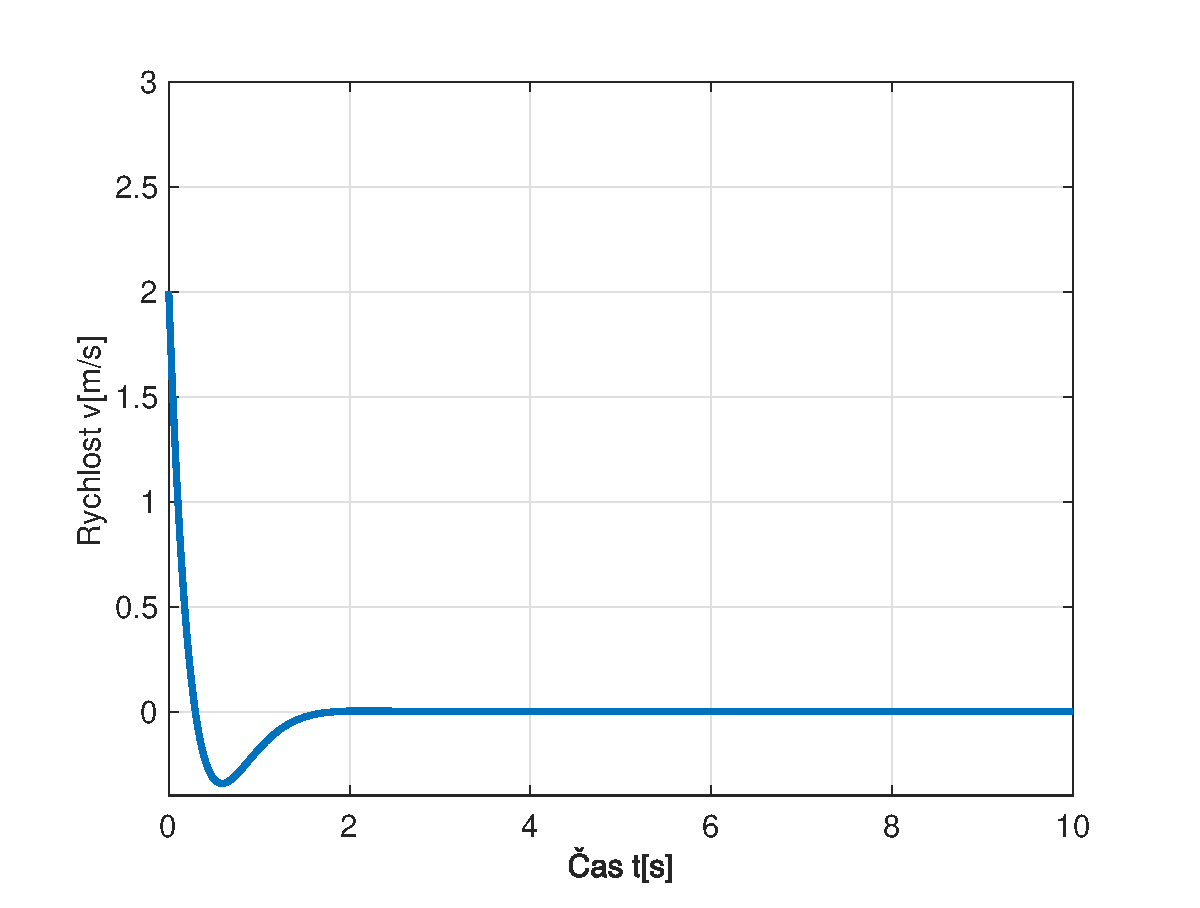
\includegraphics[width=\textwidth]{ARI_HW_0_2_1.eps}
            \caption{Časová odezva $x_1$}
        \end{subfigure}
        ~
        \begin{subfigure}[b]{0.45\textwidth}
            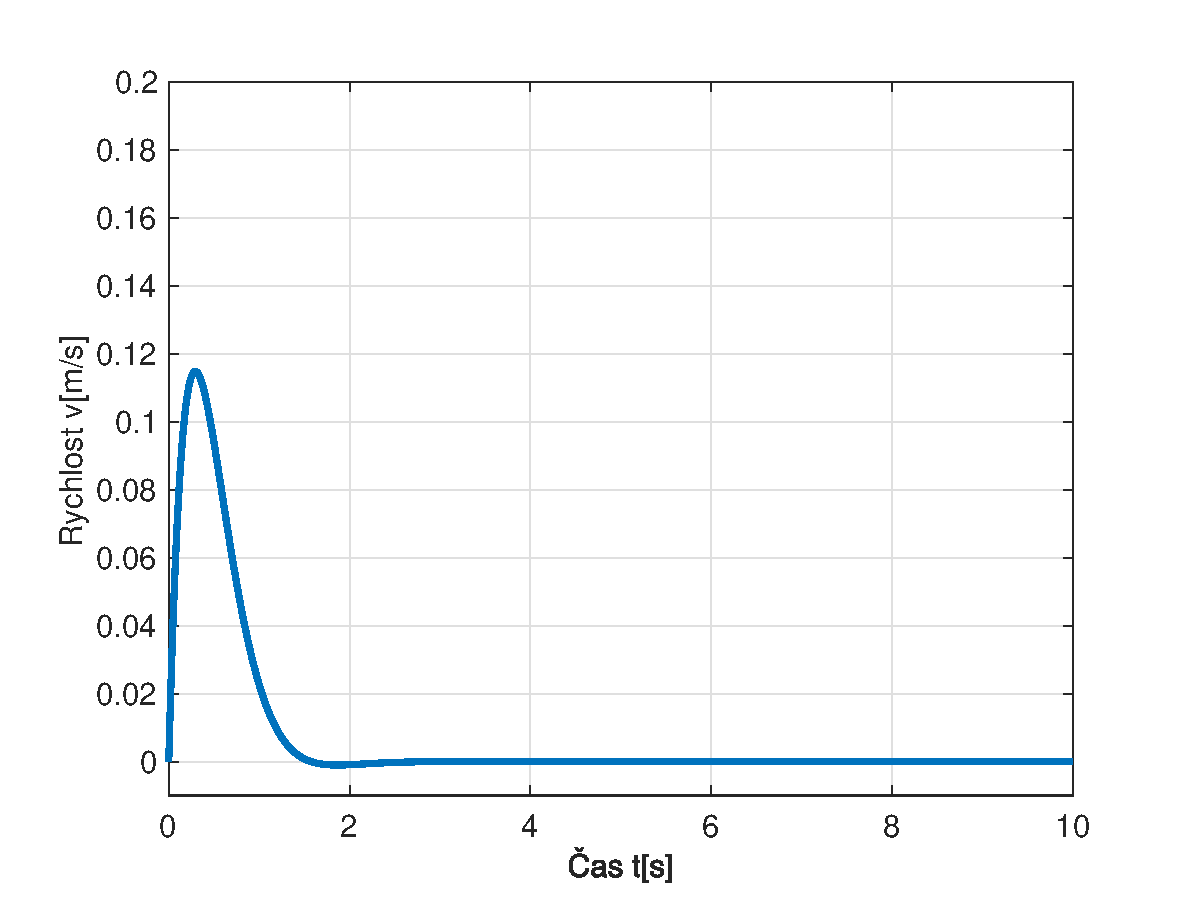
\includegraphics[width=\textwidth]{ARI_HW_0_2_2.eps}
            \caption{Časová odezva $x_2$}
        \end{subfigure}
    \end{figure}
    
\end{enumerate}
%----------------------------------------------------------------------------------------------------
%3
\hw{}
\begin{align*}
    \dot{x_1} &= x_2\\
    \dot{x_2} &= -2 sin(x_1) - \frac{1}{10}x_2+u\\
    y &= x_1\\
\end{align*}

\begin{enumerate}
    \item Rovnovážný pracovní bod P systému pro $u_p(t)$=2
    \begin{align*}
        0 &= x_2\\
        0 &= -2 sin(x_1) - \frac{1}{10}x_2+u\\
    \end{align*}
    \[P = \mat{\frac{\pi}{2}+2k\pi & 0 & \frac{\pi}{2}+2k\pi}, k \in \mathbb{Z}\]

    \item Linearizece modelu v pracovním bodě P
    \begin{align*}
        \Delta \dot x(t) &= A \cdot \Delta x(t) + B \cdot \Delta u(t)\\
        \Delta y(t) &= C \dot \Delta x(t) + D \cdot \Delta u(t)\\
        \\
        A &= \mat{0 & 1\\ -2cos(x_1) & -\frac{1}{10}} = \mat{0 & 1 \\ 0 & -\frac{1}{10}}\\
        B &= \mat{0\\1}\\
        C &= \mat{1 & 0}\\
        D &= \mat{0}\\
    \end{align*}


    \item Model systému
        \begin{figure}[H]
        \centering
        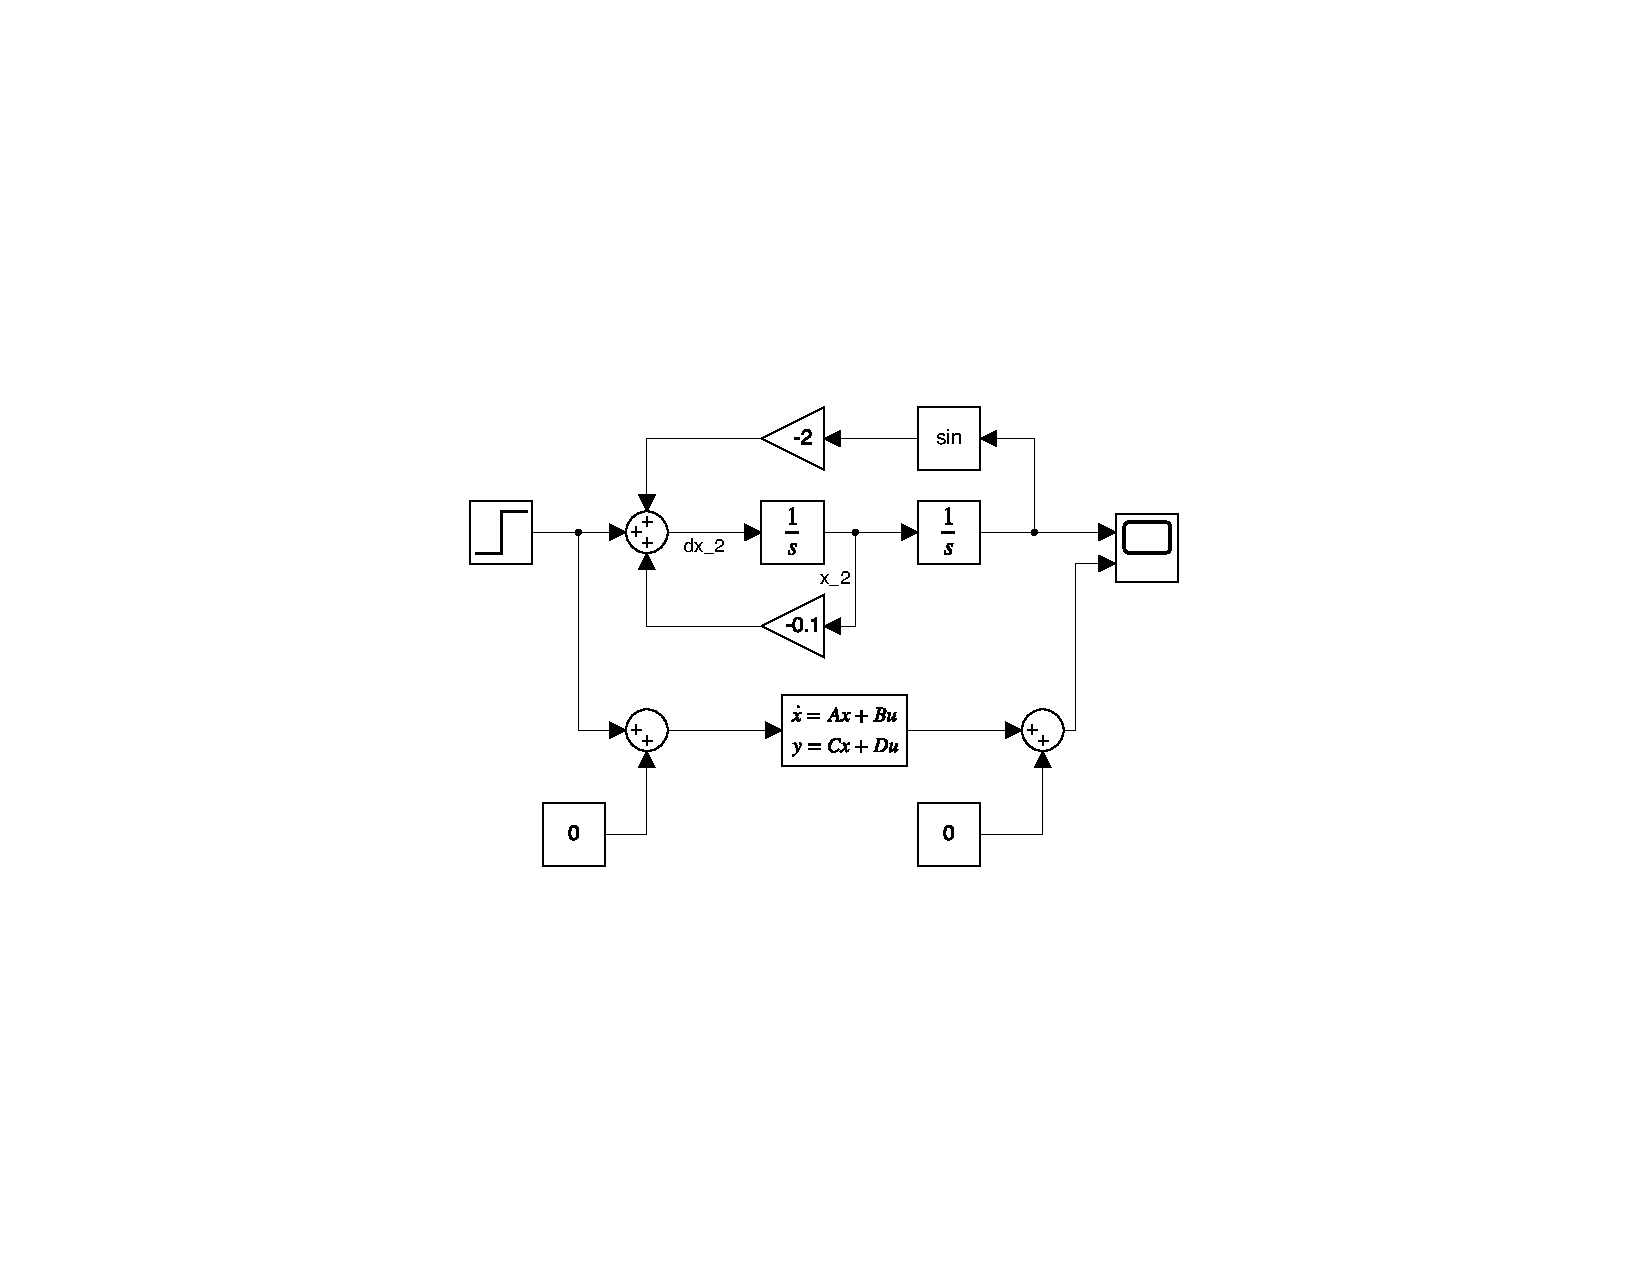
\includegraphics[clip,trim=6.1cm 6.8cm 6.1cm 6.8cm, width=1.00\textwidth]{ARI_HW_0.pdf}
        \caption{Model 1}
    \end{figure}


    \begin{figure}[H]
        \centering
        \begin{subfigure}[b]{0.45\textwidth}
            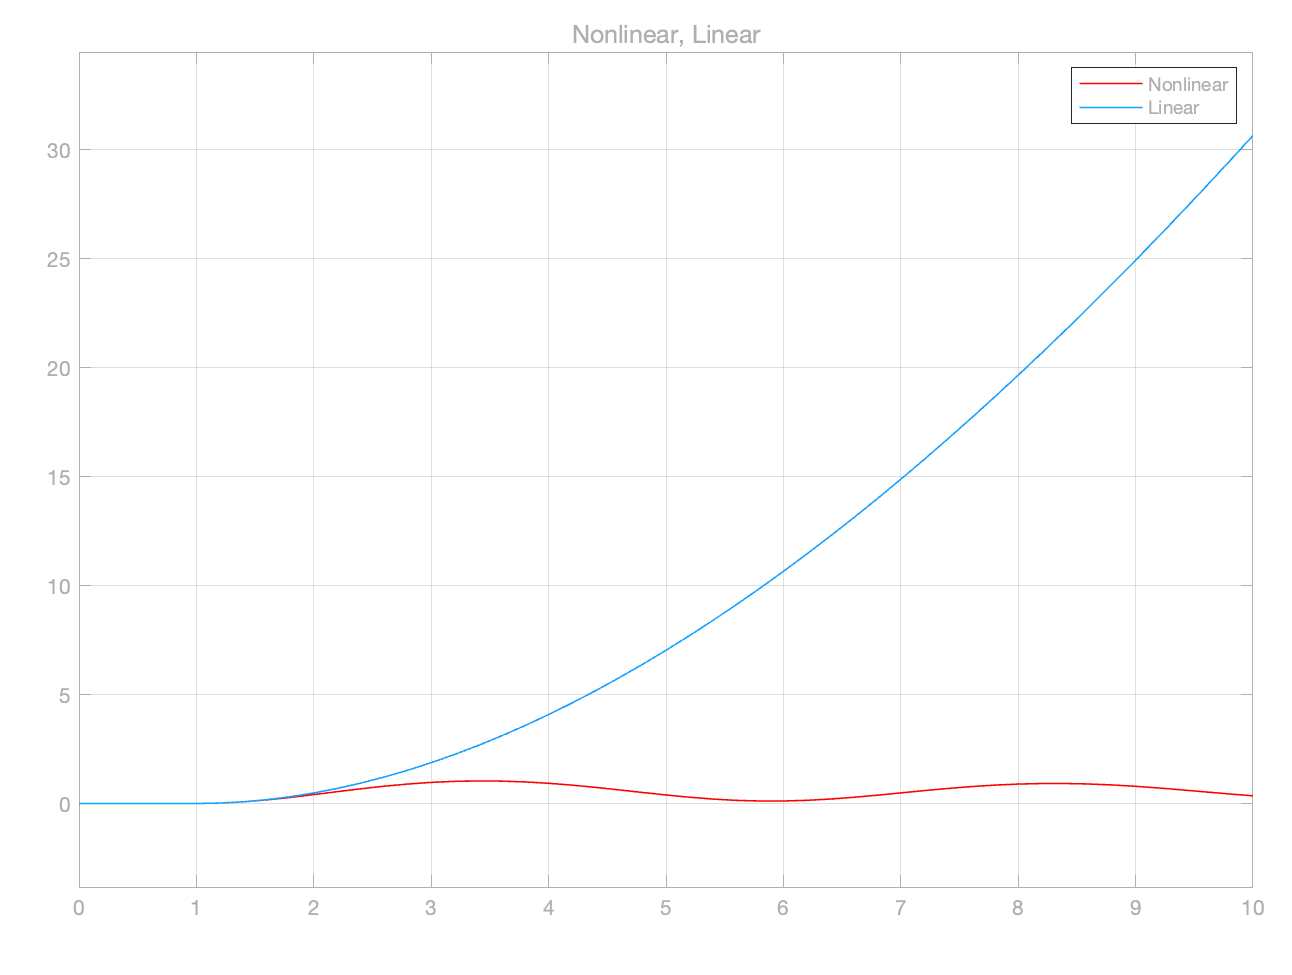
\includegraphics[width=\textwidth]{ARI_HW_0_3_linear.eps}
            \caption{Odezva na skok $u=1$}
        \end{subfigure}
        ~
        \begin{subfigure}[b]{0.45\textwidth}
            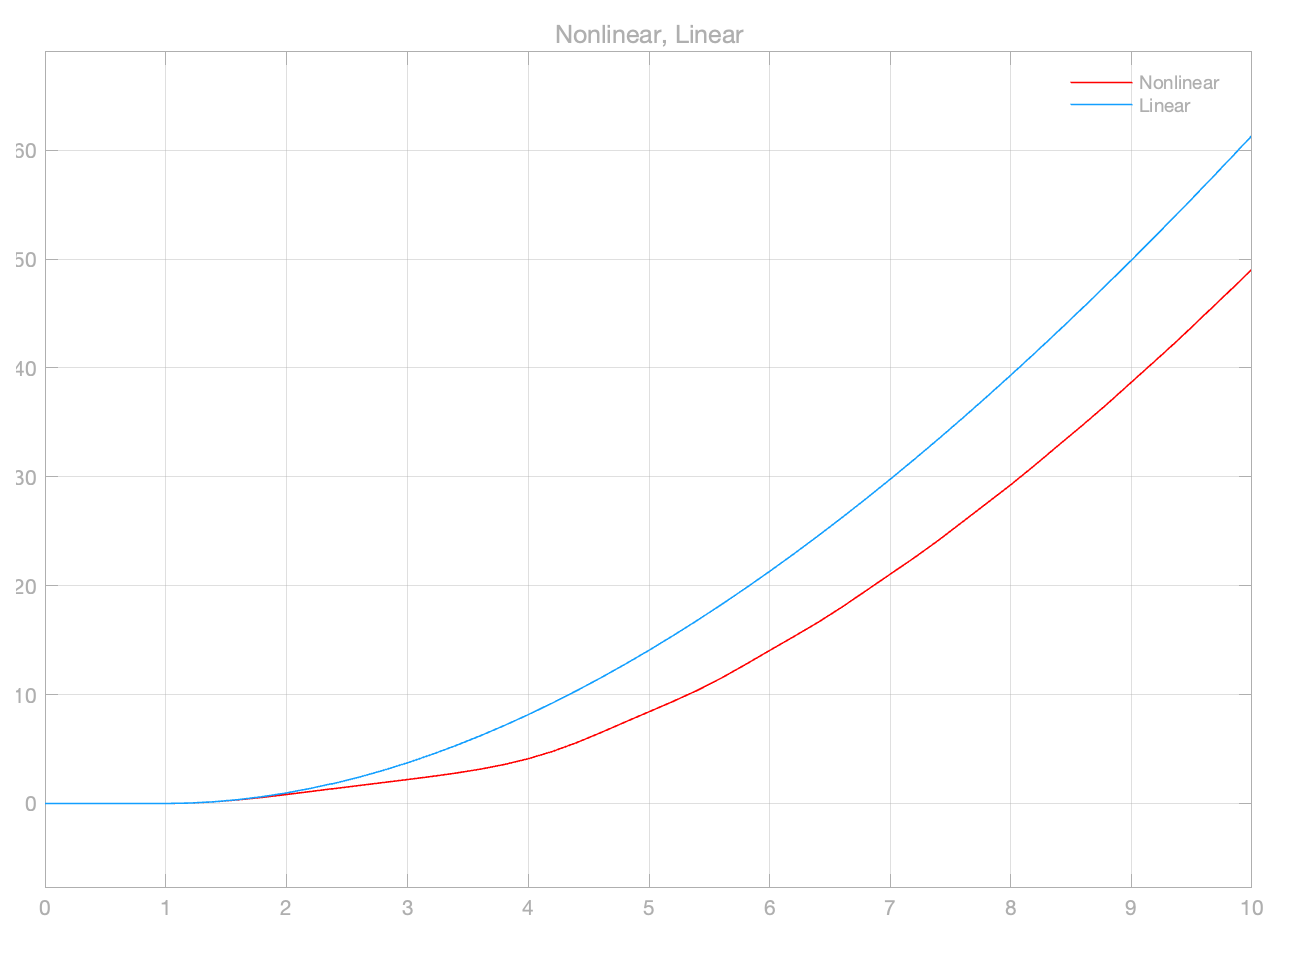
\includegraphics[width=\textwidth]{ARI_HW_0_3_NonLinear.eps}
            \caption{Odezva na skok $u=2.001$}
        \end{subfigure}
    \end{figure}
    
\end{enumerate}

%----------------------------------------------------------------------------------------------------
%4
\hw{}
\begin{enumerate}
    \item Asymptotická frekvenčí charakteristika

    \begin{figure}[H]
        \centering
        \begin{subfigure}[b]{0.45\textwidth}
            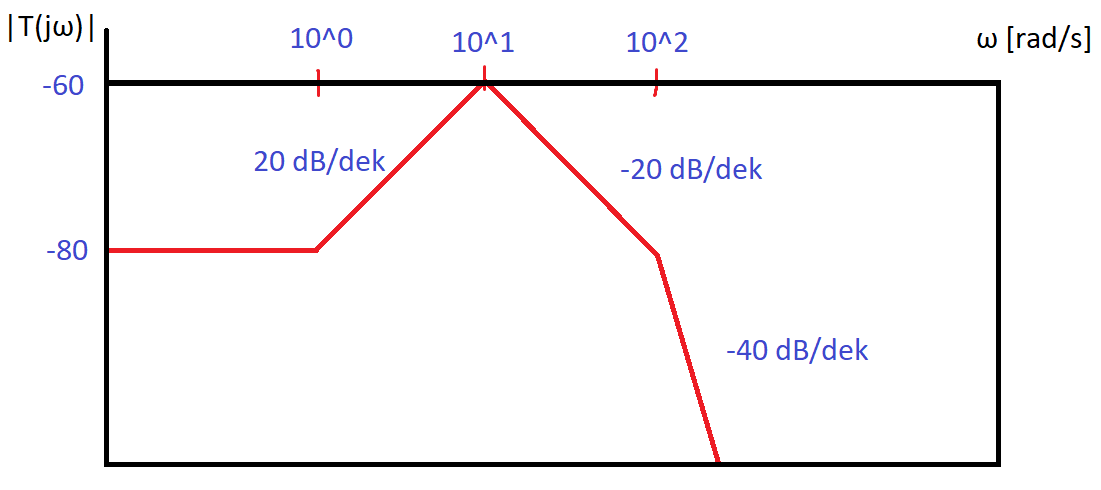
\includegraphics[width=\textwidth]{Bode_1.png}
            \caption{Amplitudová frekvenční charakteristika}
        \end{subfigure}
        ~
        \begin{subfigure}[b]{0.45\textwidth}
            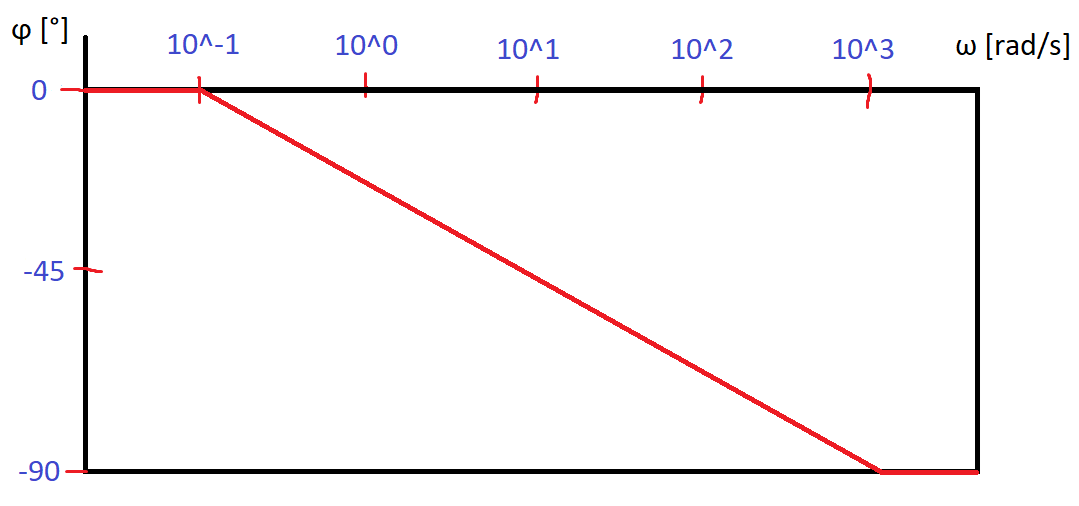
\includegraphics[width=\textwidth]{Bode_2.png}
            \caption{Fázová frekvenční charakteristika}
        \end{subfigure}
    \end{figure}

    \item Sestavení rovnice

    \begin{align*}
        G(s) &= -\frac{(1-j\frac{\omega}{10^{-1}})(1+j\frac{\omega}{10^{1}})}{(1+j\frac{\omega}{10^{-3}})(1+j\frac{\omega}{10^{3}})} = \frac{(s-10^{-1})(s+10)}{(s+10^{-3})(s+10^3)}
    \end{align*}
    
\end{enumerate}

%----------------------------------------------------------------------------------------------------
%5
\hw{}
\begin{align*}
    H(s) &= C(sI-A)^{-1}B = \mat{4 & 0 & 0 & 0} \pmat{\mat{s & 0 & 0 & 0\\
                                                      0 & s & 0 & 0\\
                                                      0 & 0 & s & 0\\
                                                      0 & 0 & 0 & s}
                            - \mat{-4 & 2 & 0 & 0\\
                                   -6 & 4 & 0 & 0\\
                                   -3 & 3 & 2 & -2\\
                                   -9 & 9 & 2 & -3}}^{-1} \mat{1\\0,5\\0\\-1}\\
    &= \frac{4(s+2)(s-2)(s-3)}{(s+2)^2(s-2)^2}
\end{align*}

%----------------------------------------------------------------------------------------------------
%6
\hw{}
Systém je stabilní pokud jeho póly přenosu mají zápornou reálnou část
\begin{align*}
    det(sI-A) &= \vmat{s-1 & 0 & 0\\-2 & s+2 & 2\\ -1 & -2 & s} = (s-1)(s+2)s+2(s-1)2=\\
    &= s^3+s^2+2s-4 = (s-1)(s+1\pm i \sqrt{3})
\end{align*}

%----------------------------------------------------------------------------------------------------
%7
\hw{}
\begin{enumerate}
    \item Vhodně zvolená vzorkovací perioda $T_s = 0.1$s\\
    \\
    $G(z)= \frac{0.05642z-0:07695}{z^2-1.401z+0.4493}$

    \item Nevhodně zvolená vzorkovací perioda $T_s = 3$s\\
    \\
    $G(z) = \frac{-0.3954 z - 0.01185}{  z^2 - 0.04979 z + 3.775e-11}$


\end{enumerate}

%----------------------------------------------------------------------------------------------------
%8
\hw{}
\begin{enumerate}
    \item Stabilní (-$\frac{2}{5}$, -1, -3), statický, nekmitavý
    \item Nestabilní ($\frac{-1\pm \sqrt{17}}{4}$, statický, nekmitavý
    \item Nestabilní (0), astatický, nekmitavý
    \item Nestabilní ($\pm \sqrt{2}$), statický, nekmitavý
\end{enumerate}
%----------------------------------------------------------------------------------------------------
%9
\hw{}
\begin{enumerate}
    \item $H = G_1 + G_2 = \frac{s^2+01}{s^2+s}$
    \item $H = G_1 \cdot G_2 = \frac{s-1}{s^2+s}$

    \item $H = \frac{y(s)}{r(s)}; G=G_1 \cdot G_2$\\
    $y(s) = G(r(s)-y(s)) \rightarrow G(y(s))+y(s)=G(r(s)) \rightarrow \\y(s)(1+G)=Gr(s) \rightarrow H=\frac{y(s)}{r(s)}=\frac{G}{1+G}=\frac{\frac{s-1}{s^2+s}}{1+\frac{s-1}{s^2+s}}=\frac{s-1}{s^2+2s-1}$    

    \item $H = \frac{y(s)}{r(s)}$\\
    $y(s) = G_1(r(s)-y(s)G_2) \rightarrow G_1G_2y(s) + y(s) = G_1r(s) \rightarrow \\ y(s)(1+G_1G_2)=G_1r(s) \rightarrow H=\frac{y(s)}{r(s)}=\frac{G_1}{1+G_1G_2} = \frac{\frac{s-1}{s+1}}{1+\frac{s-1}{s+1} \frac{1}{s}}=\frac{s^2-s}{s^2+2s-1}$

\end{enumerate}
%----------------------------------------------------------------------------------------------------
%10
\hw{}


\begin{enumerate}
    \item Přenos systému
    \begin{align*}
        3Y(z) - Y(z)z^{-1} + \frac{1}{2}Y(z)z^{-2} &= U(z)z^{-1} - U(z)z^{-2}\\
        Y(z)(3-z^{-1} + \frac{1}{2}z^{-2} &= U(z)(z^{-1} - z^{-2})\\
        H(z) & = \frac{Y(z)}{U(z)} = \frac{z^{-1} - z^{-2}}{3 - z^{-1} + \frac{1}{2}z^{-2}}
    \end{align*}

    \item Stabilita systému
    \begin{align*}
    3z^{2}-z+\frac{1}{2} &= 0 \rightarrow\\
    \frac{1 \pm \sqrt{-5}}{6} &= \frac{1}{6} \pm \frac{\sqrt{-5}}{6}i
    \end{align*}
    Póly systému jsou v jednotokové kružnici stability, takže systém je stabilní

    \item Model a odezva systému

     \begin{figure}[H]
        \centering
        \begin{subfigure}[b]{0.45\textwidth}
            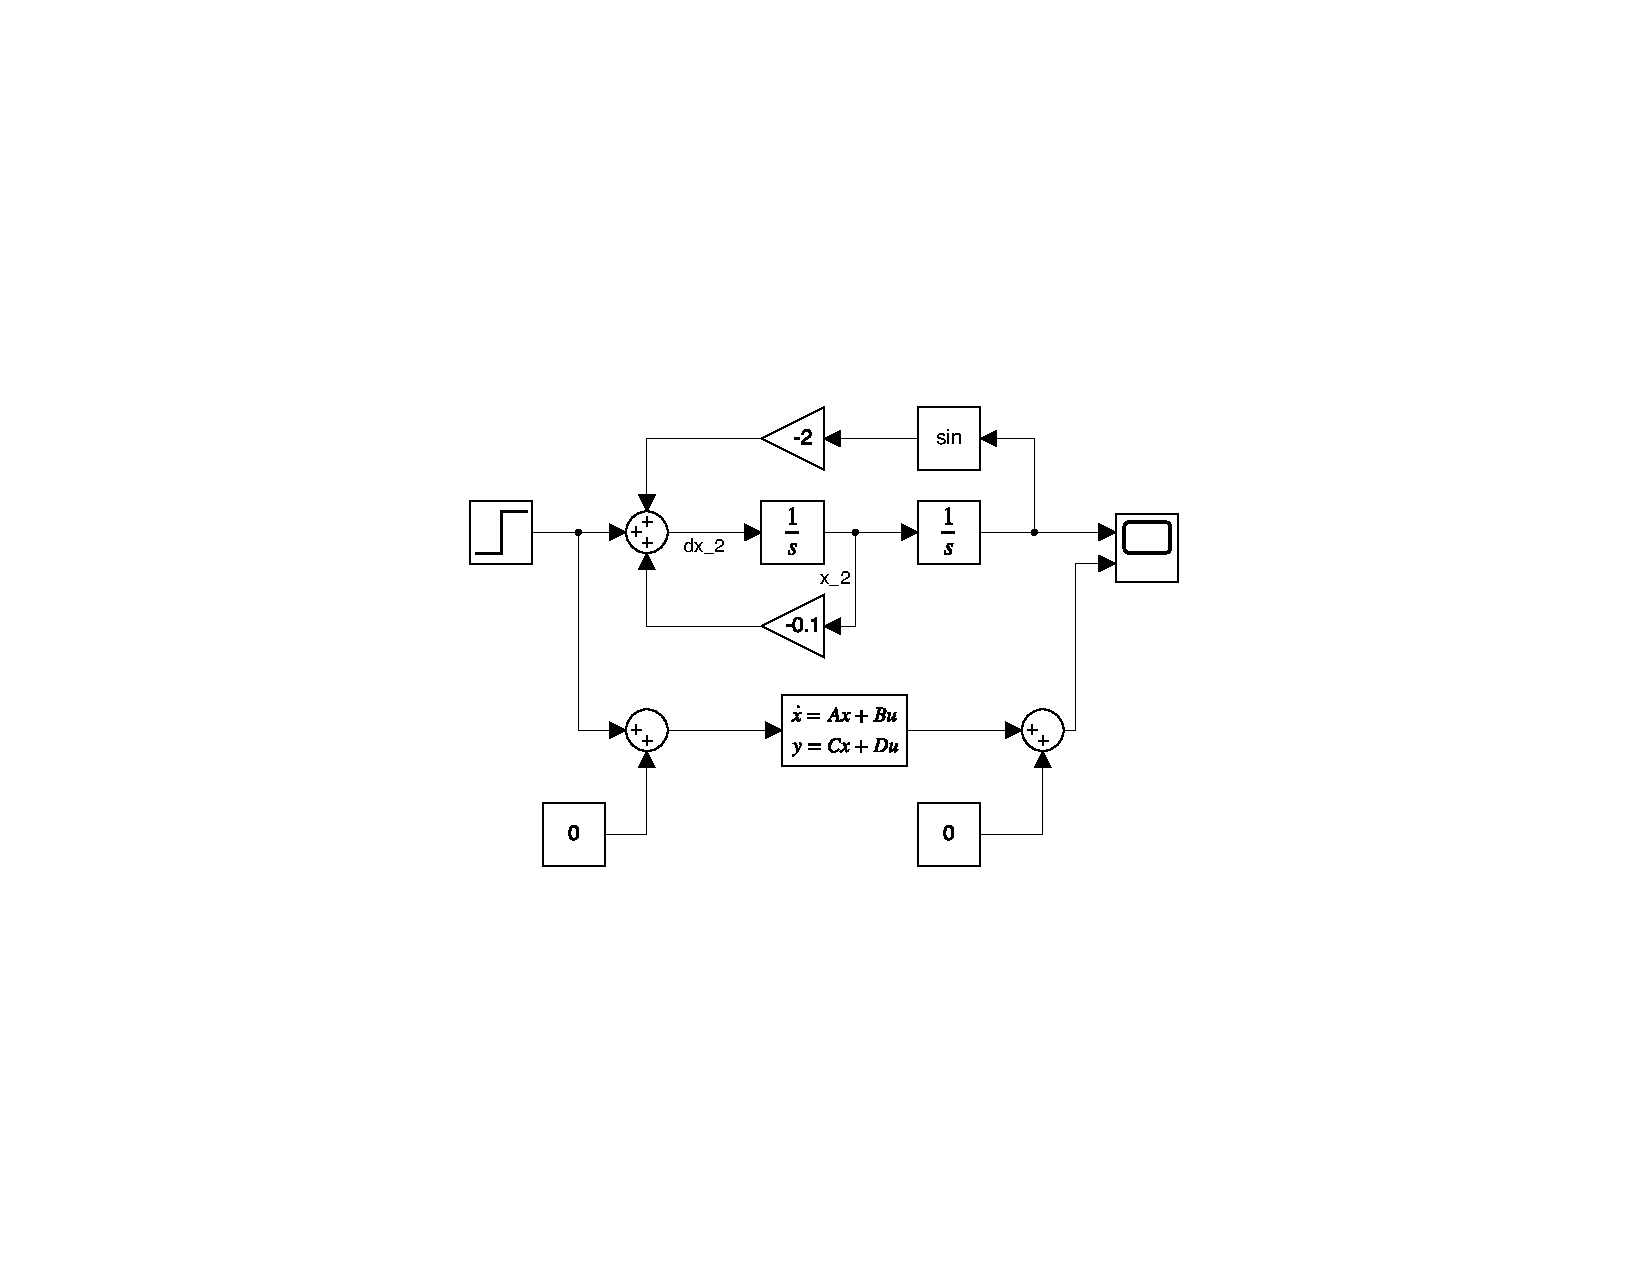
\includegraphics[clip,trim=6.1cm 6.8cm 6.1cm 6.8cm, width=1.00\textwidth]{ARI_HW_0.pdf}
            \caption{Model systému}
        \end{subfigure}
        ~
        \begin{subfigure}[b]{0.45\textwidth}
            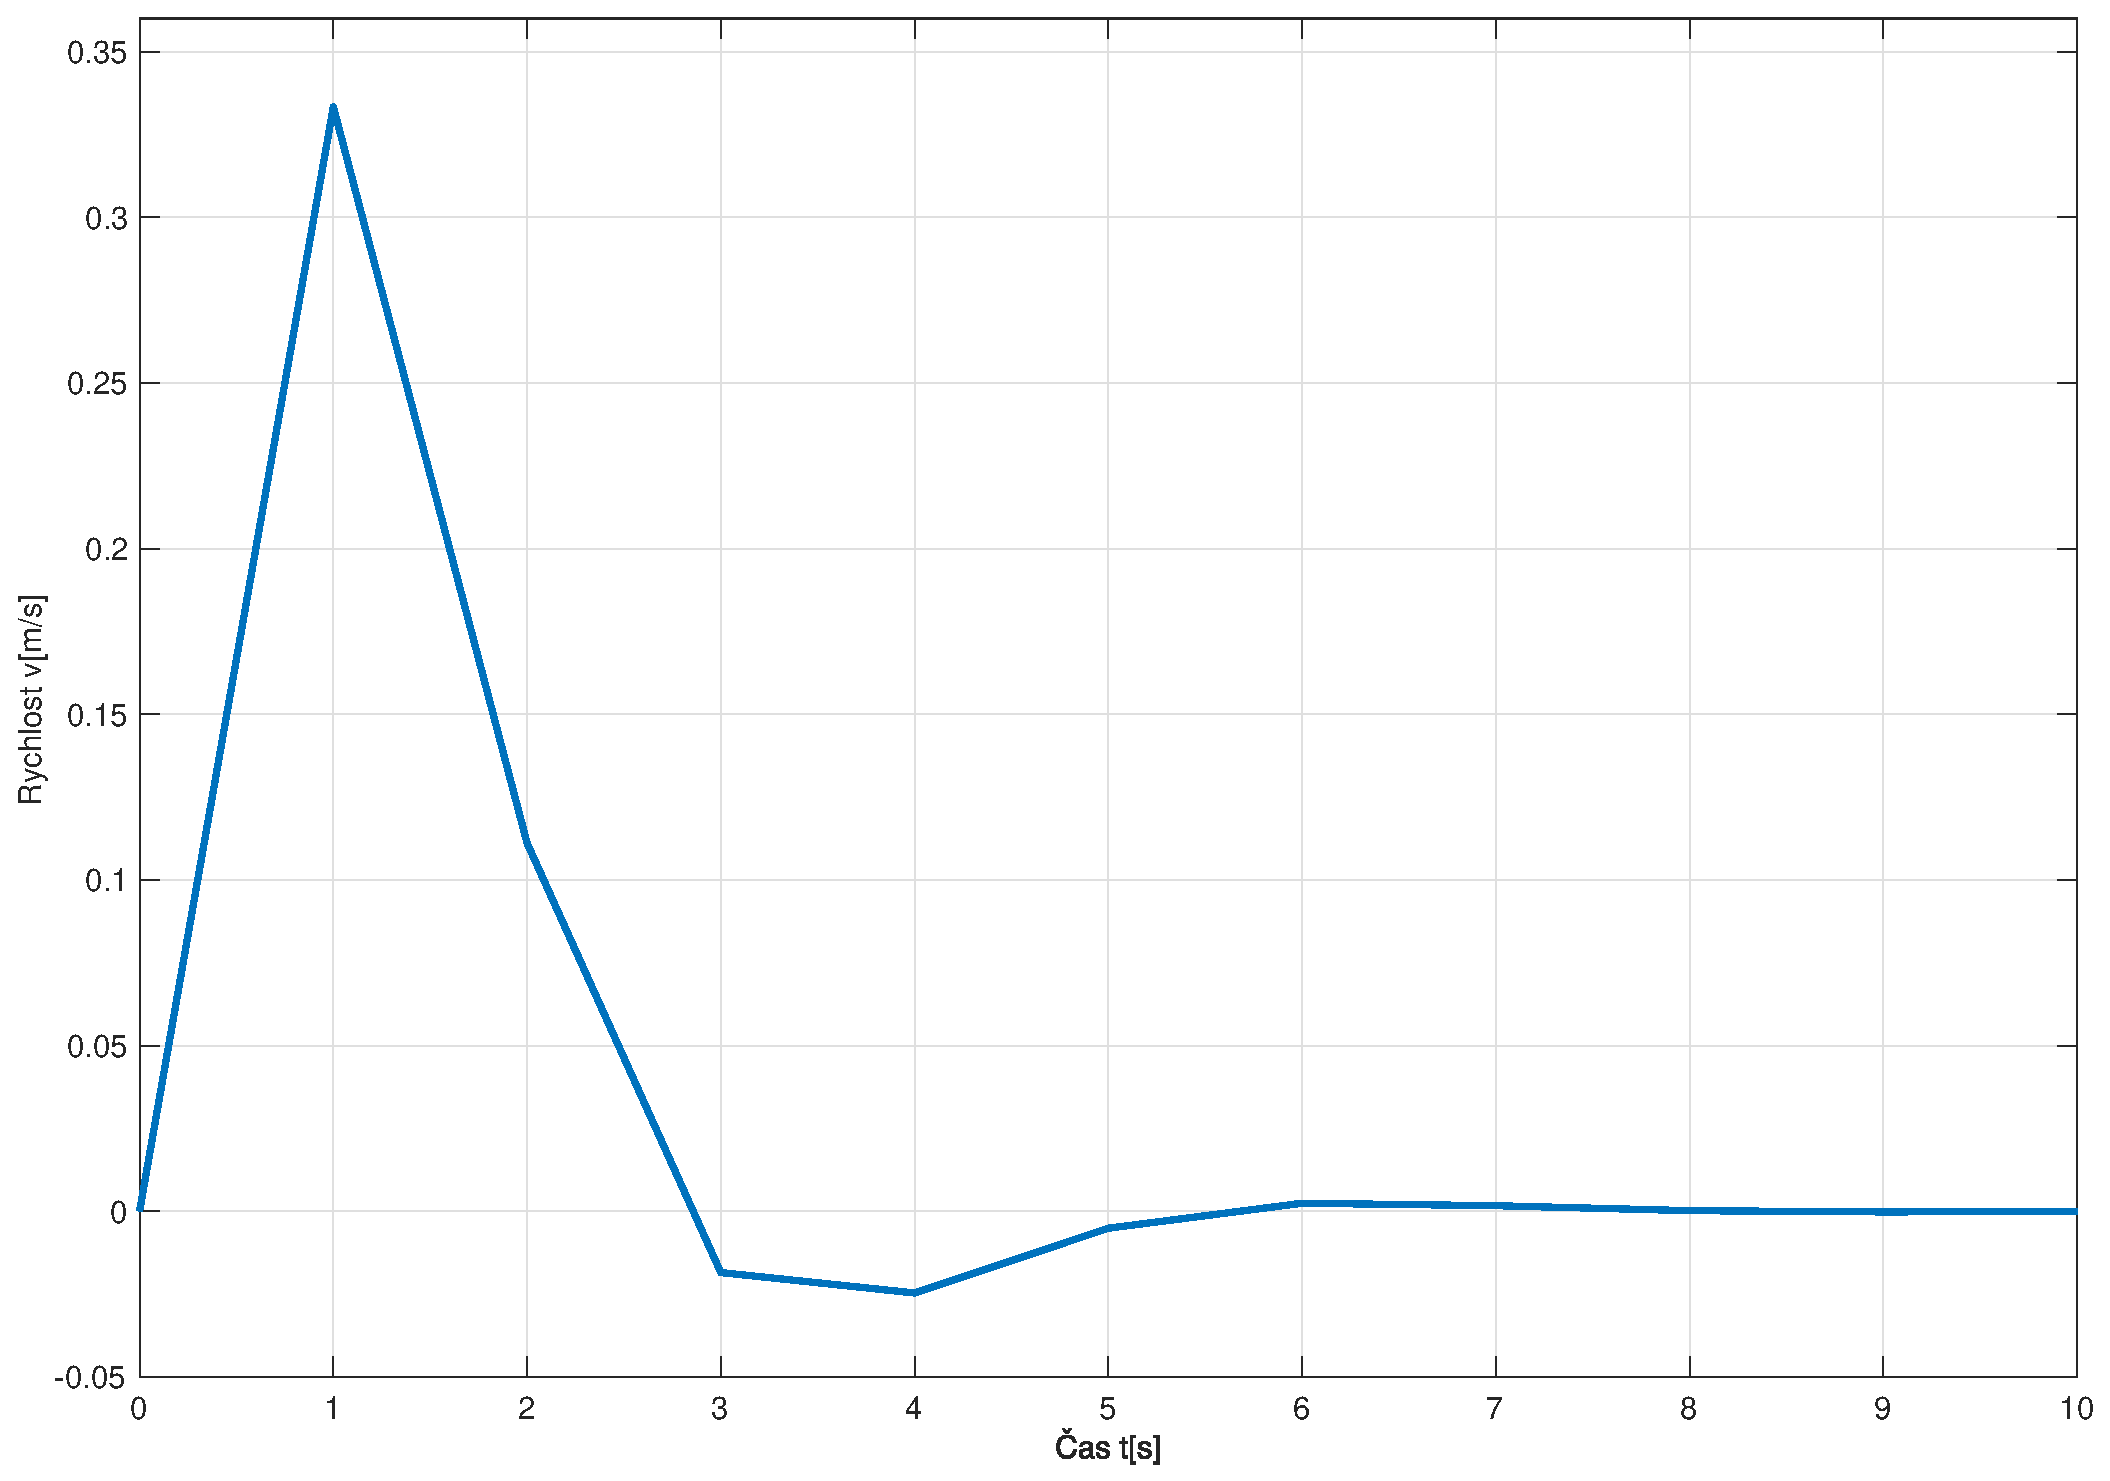
\includegraphics[width=\textwidth]{Odezva_10.eps}
            \caption{Odezva systému}
        \end{subfigure}
    \end{figure}
    
\end{enumerate}
%----------------------------------------------------------------------------------------------------
%11
\hw{}
\begin{enumerate}
    \item a-f; b-d; c-e
    \item Impulz $h(t)$; Skok $w(t)$\\
    $w(t) = \int_{-\inf}^{t} h(t) dt$\\
    $h(t)=\frac{dw(t)}{dt}$
\end{enumerate}
%----------------------------------------------------------------------------------------------------
%12
\hw{}
\begin{enumerate}
    \item a-f; b-d; c-e
    \item Pro fázi -45\degree má systém zesílení -3 dB
\end{enumerate}

\end{document}
